\documentclass[12pt]{article}
\usepackage[utf8]{inputenc}
\usepackage[T1]{fontenc}
\usepackage{fontspec}
\setmainfont{Times New Roman}
\newfontfamily\hackfont{Hack}
\usepackage{titlesec}
\usepackage{fancyhdr}
\usepackage{listings}
\usepackage{xcolor}
\usepackage{graphicx}
\usepackage{longtable}
\usepackage{caption}
\usepackage{hyperref}
\usepackage{setspace}
\usepackage{geometry}
\geometry{a4paper, margin=1in}
\hypersetup{colorlinks=true, linkcolor=blue, urlcolor=blue}
\renewcommand{\contentsname}{Table of Contents}

\pagestyle{fancy}
\fancyhf{} 							% Header Middle
\rhead{VLSI Design Lab}
\lhead{Lab-03: Adder Circuit}
\rfoot{\thepage}

\begin{document}

\begin{titlepage}					% Cover Start
\begin{center}
    
\includegraphics[width=0.35\textwidth]{logo.png} \\
    \vspace{0.5cm}
    \textbf{\Huge \textcolor{cyan}{NOTRE DAME} \textcolor{cyan}{UNIVERSITY}} \\
    \vspace{0.5cm}
    \textbf{\Huge \textcolor{orange}{BANGLADESH}} \\
    
    \vspace{0.9cm}
    \textbf{\Huge \underline{VLSI Design Lab Report-03}} \\
    
    \vspace{1.5em}
    \begin{flushleft}
    	\textbf{\Large Course Code: CSE-4218} \\
		\vspace{0.3cm}        
        \textbf{\Large Course Title: VLSI Design Lab} \\
        \vspace{0.3cm}
        \textbf{\Large Experiment Name: Implementing Adder Circuit} \\        
    \end{flushleft}
    
    \vspace{1em}
    \begin{flushleft}
        \textbf{\Huge \textcolor{blue}{Submitted by:}} \\
        \vspace{0.3cm}
        \textbf{\Large Name: Istiak Alam} \\
        \vspace{0.3cm}
        \textbf{\Large ID: 0692230005101005} \\
		\vspace{0.3cm}        
        \textbf{\Large Batch: CSE-20} \\
        \vspace{0.5cm}
        \textbf{\Large Submission Date: }{\Large \textbf{\today}\par}
    \end{flushleft}
    \vfill
    \begin{flushleft}
        \textbf{\Huge \textcolor{blue}{Submitted to:}} \\
        \vspace{0.3cm}
        \textbf{\Large Nfisa Tabassum,} \\
        \vspace{0.3cm}
        \textbf{\Large Lecturer, Dept. of CSE} \\
        \vspace{0.3cm}
        \textbf{\Large Notre Dame University Bangladesh}
    \end{flushleft}
\end{center}
\end{titlepage}						% Cover End

\tableofcontents
\thispagestyle{empty}
\clearpage
\pagenumbering{arabic}

\section*{\center Abstract}
This laboratory experiment presents the design and implementation of Adder Circuit using the DSCH2 schematic simulation tool. The circuits were designed following standard CMOS pull-up and pull-down network principles. For each logic function, the corresponding truth table was derived and verified through schematic simulation. Timing diagrams were analyzed to observe the dynamic response and switching behavior of the circuits. The experimental results confirm that the implemented CMOS designs satisfy the expected logical and temporal characteristics of the half adder circuit.


\section{Introduction}
A combinational logic circuit which is designed to add two binary digits is called as a half adder. The half adder provides the output along with a carry value (if any). The half adder circuit is designed by connecting an EX-OR gate and one AND gate. It has two input terminals and two output terminals for sum and carry.


\section{Objective}
The objectives of this VLSI-Lab experiment are as follows:
\begin{itemize}
    \item To implement Adder Circuit using CMOS logic design methodology.
    \item To design schematic-level Adder circuits using the DSCH2 tool.
    \item To verify the logical correctness of the implemented circuits using truth tables.
    \item To analyze timing diagrams to observe signal transitions and propagation behavior.
    \item To develop a clear understanding of Adder Circuit.
\end{itemize}

\section{Half Adder Function}

\subsection{Boolean Function}
\[
Sum = AB' + A'B
\]
\[
Carry= A⋅B
\]

\subsection{Truth Table}
\begin{center}
\begin{tabular}{|c|c|c|c|c|}
\hline 
A & B & Sum & Carry \\ \hline
0 & 0 & 0 & 0  \\
0 & 1 & 1 & 0  \\
1 & 0 & 1 & 0  \\
1 & 1 & 0 & 1  \\ \hline
\end{tabular}
\end{center}

\subsection{Schematic Image}
\begin{figure}[!h]
\centering
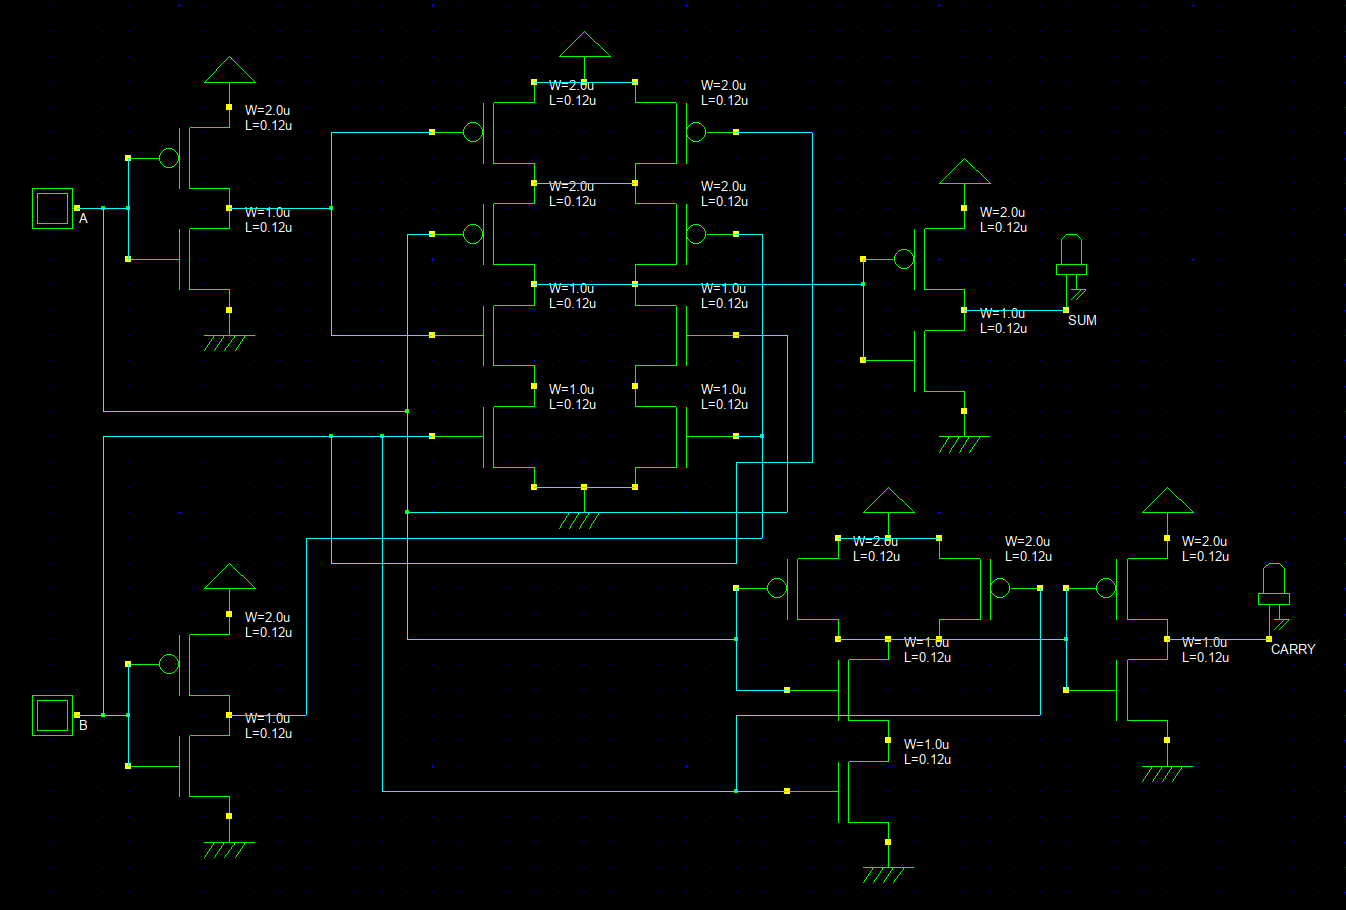
\includegraphics[width=0.8\textwidth]{Half-Adder.png}
\caption{CMOS Schematic of Half-Adder}
\end{figure}

\subsection{Timing Diagram}
\begin{figure}[!h]
\centering
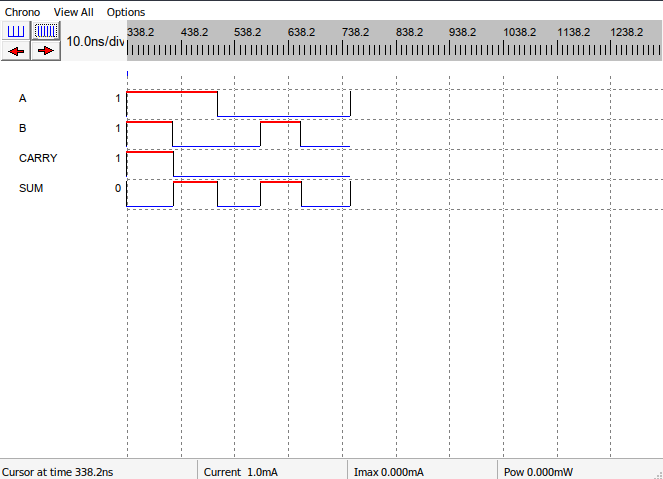
\includegraphics[width=0.7\textwidth]{Half-Adder-TD.png}
\caption{Timing Diagram of Half-Adder}
\end{figure}
  


\subsection{Observation}
The timing diagram of a half adder illustrates the sequence of operations that occur when two binary inputs are added. The diagram typically shows the timing of the XOR operation for the sum and the timing of the AND operation for the carry. The timing diagram can help in understanding the propagation delay and the timing constraints of the circuit. It is important to note that the timing diagram should be adjusted to account for the specific timing requirements of the circuit design, such as rise/fall time and maximum input frequency. 


\section{Conclusion}
Adder circuit were successfully implemented and verified using DSCH2. Truth tables and timing diagrams matched theoretical expectations, confirming correct logical and temporal behavior of each function.

\end{document}